\chapter{Instrumentation Amplifiers}

Instrumentation amplifiers are differential amplifiers just like operational amplifiers -- in fact, instrumentation amplifiers are constructed out of several operational amplifiers.
Instrumentation amplifiers, or in amps, have an extremely high input impedance.
This high input impedance is often achieved with a three op amp topology, using two of the op amps as input buffers or non-inverting amplifiers.
The in amp's input impedance is much higher than the op amp difference amplifier previously discussed, so the in amp is able to measure a differential voltage with much better accuracy.
In amps are often used to calibrate electronic instruments (hence the name \textit{instrumentation} amplifier) or to directly measure the small voltage signals from sensors (such as pressure transducers), voltage references, test equipment, etc.

While in amps can be constructed out of discrete op amps and resistors, the input op amps and all the resistors must be highly matched in order to minimize undesirable characteristics such as input offset voltage, common mode gain, etc.
As a result, in amps are usually constructed in integrated circuit form.

\section{Three op amp topology instrumentation amplifier}
\begin{center}
	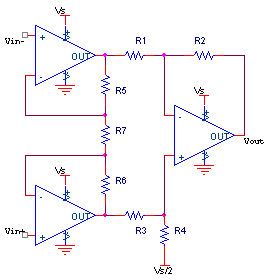
\includegraphics{schematics/threeinamp.PNG}
\end{center}
This is the standard, symmetric topology using three op amps.
To maintain symmetry (which, in this case, ensures each input voltage is amplified by the same amount), we must have

\begin{equation}
R_{5} = R_{6}
\end{equation}

\begin{equation}
R_{1} = R_{3}
\end{equation}

\begin{equation}
R_{2} = R_{4}
\end{equation}

\noindent The input differential voltage is

\begin{equation}
v_{diff} = v_{in+}-v_{in-}
\end{equation}

\noindent and it is the voltage across $R_{7}$ since the voltages at the inverting inputs of the input op amps are equal to the input voltages. The current through $R_{7}$ is thus

\begin{equation}
i_{R7} = \frac{v_{diff}}{R_{7}}
\end{equation}

The differential voltage between the two input op amps' outputs (call it $v_{o1}$) is

\begin{equation}
v_{o1} = i_{R7}(R_{5}+R_{6}+R_{7}) = i_{R7}(2R_{5}+R_{7}) = v_{diff}(1+2\frac{R_{5}}{R_{7}})
\end{equation}

The output op amp is configured as a difference amplifier with $v_{o1}$ as the input so the overall gain $A_{v}$ is

\textcolor{red}{
\begin{equation}
A_{v} = \frac{R_{2}}{R_{1}}(1+2\frac{R_{5}}{R_{7}})
\label{eq:threeinamp}
\end{equation}
}

$R_{5}$ and $R_{6}$ can be shorted and $R_{7}$ removed (replaced with an open circuit) to reduce the number of resistors -- this configures the input op amps as buffers. The disadvantage, of course, is that the output op amp must be configured with a higher gain in order to achieve the same overall gain, which will reduce the in amp's bandwidth.

\section{Two op amp topology instrumentation amplifier}
\begin{center}
	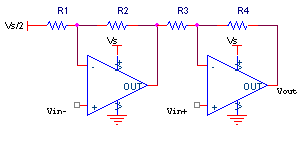
\includegraphics{schematics/twoinamp.PNG}
\end{center}
This in amp topology is less common but uses only two op amps, which can be useful to minimize the number of op amps used in the application circuit or to minimize power consumption. As with the three op amp topology, resistors must be matched:

\begin{equation}
R_{1} = R_{4}
\end{equation}

\begin{equation}
R_{2} = R_{3}
\end{equation}

\noindent The transfer function is

\textcolor{red}{
\begin{equation}
A_{v} = 1+\frac{R_{1}}{R_{2}}
\label{eq:twoinamp}
\end{equation}
}

Unfortunately, this topology requires the $v_{in-}$ op amp to be used with less than unity gain (so it may be unstable) and the $v_{in-}$ signal has a higher propagation delay than the $v_{in+}$ signal. Depending on the application circuit and the op amps available, the three op amp topology may have to be used instead.